
\begin{frame}{Motivación 1/2}

    \begin{figure}[ht]
        \begin{center}
            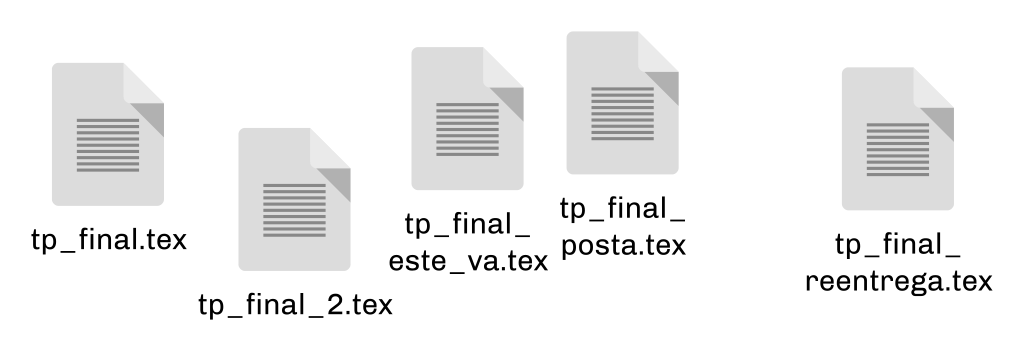
\includegraphics[height=1.5in]{images/caos.png}
        \end{center}
    \end{figure}

    \pause
    \begin{figure}[ht]
        \begin{center}
            
\includegraphics[height=1.5in]{images/horror.png}
        \end{center}
    \end{figure}
\end{frame}
\begin{frame}{Motivación 2/2}

    \begin{block}{Trabajando en grupo}
        \begin{itemize}
            \item Enviar cambios por mail, o
            \pause
            \item Enviar archivos por Discord, o
            \pause
            \item Sincronizar cambios por Google Docs.
        \end{itemize}
    \end{block}

    \pause
    \begin{figure}[h]
        \begin{center}
            
\includegraphics[height=1.5in]{images/horror.png}
        \end{center}
    \end{figure}

\end{frame}

\begin{frame}{¿Qué es un Sistema de Control de Versiones?}

	\begin{block}{}
 \begin{enumerate}
     \item Programas que permiten \textbf{manejar los cambios} en el código fuente de un proyecto a lo largo del tiempo.
     \item Llevan un \textbf{seguimiento} de las modificaciones que hacemos, y en caso de que nos equivoquemos, es posible volver atrás y comparar el código actual con versiones anteriores para ayudar a arreglar el error.
     \item Permiten que distintas personas modifiquen el código a la vez y \textbf{compartan los cambios}.
 \end{enumerate}

	\end{block}

 %   \pause
 %    \begin{resumen}{Es decir, permiten...}
 %        \begin{itemize}
 %            \item Arreglar \textit{accidentes} y volver a versiones anteriores del código.
 %            \item Compartir código con otras personas.
 %        \end{itemize}
	% \end{resumen}

\end{frame}

\begin{frame}{¿Qué es Git? 1/3}

	\begin{block}{}
 \begin{itemize}
     	\item Sistema de Control de Versiones \textbf{distribuido y de código abierto}.
  
        \item Con énfasis en la \textbf{performance} (para manejar proyectos muy grandes), \textbf{seguridad} y \textbf{flexibilidad}.
        
        \item Amplio conjunto de comandos que permiten realizar operaciones de alto y bajo nivel.

        \item Mantiene una copia local completa del proyecto.
 \end{itemize}

	\end{block}

    \begin{figure}[ht]
        \begin{center}
            
\includegraphics[height=1.5in]{images/logo-git.png}
        \end{center}
    \end{figure}
\end{frame}

\begin{frame}{¿Qué es Git? 2/3}
    \begin{center}
        \begin{block}{GIT - the stupid content tracker}

            "git" can mean anything, depending on your mood.
            
             - \textbf{random three-letter combination that is pronounceable}, and not actually used by any common UNIX command.  The fact that it is a mispronunciation of "get" may or may not be relevant.\newline
             - \textbf{stupid}. contemptible and despicable. simple. Take your pick from the dictionary of slang.\newline
             - \textbf{"global information tracker"}: you're in a good mood, and it actually works for you. Angels sing, and a light suddenly fills the room. \newline
             - \textbf{"goddamn idiotic truckload of sh*t"}: when it breaks
        \end{block}
    \end{center}
    \pause
    \textit{ - Mensaje del commit de Linus Torvalds agregando el README al repositorio Git de Git (uf)}
    
\end{frame}


\begin{frame}{¿Qué es Git? 3/3}
\begin{center}
    \begin{block} {¿Y entonces?}
        \begin{itemize}
            \item Es un programa que nos permite hacer un seguimiento del estado de un \textbf{repositorio}.
            \pause
            \item Se puede usar de manera local, o subir un \textbf{repositorio} a internet y usarlo de manera colaborativa. 
        \end{itemize}
    \end{block}
\end{center}
\pause
    \begin{block}{¿Repositorio? ¿Y eso?}
    \begin{itemize}
        \pause
        \item La unidad básica donde guardaremos todos los elementos de nuestro proyecto.
        \pause
        \item Es un directorio o carpeta.
        \pause
        \item La idea es que nuestro proyecto, y todos los archivos que lo contengan, existan dentro de este \textbf{repositorio}.
        \pause
        \item Sabemos que una carpeta es un \textbf{repositorio} de Git porque tiene dentro una subcarpeta \textit{.git}.
    \end{itemize}

    \end{block}
    
\end{frame}

\begin{frame}[fragile]{Configuraciones iniciales}

    \begin{block}{Tu identidad}
        Es importante establecer nuestro \textbf{nombre y email} en nuestro repositorio, ya que estos van a ir asociados con los cambios que hagamos:

        \vspace{0.5em}

        \texttt{git config --global user.name "Guybrush Threepwood"}

        \texttt{git config --global user.email guybrush@example.com}


    También se puede omitir el flag \texttt{--global} para que las credenciales apliquen solo al repositorio en el que estamos trabajando.
        \end{block}
\end{frame}

\begin{frame}[t]{Creando un repositorio}
    \begin{comando}
        git init
    \end{comando}

    \pause
    \begin{block}{}
        Crea un repositorio local.
        \begin{enumerate}
            \item Nos paramos en el directorio que queremos convertir en un repositorio.
            \item Ejecutamos \texttt{git init}.
        \end{enumerate}
        Esto crea un subdirectorio \textit{.git} que tiene todos los archivos necesarios de Git.
    \end{block}
    \pause
    \begin{ejercicio}{Ejercicio}
        Creen un directorio o carpeta nueva. Dentro de ella, ejecuten \texttt{git init}. Recuerden los comandos de bash \textit{cd, ls}.
    \end{ejercicio}
\end{frame}

\begin{frame}{¿Directorio o repositorio?}
    \begin{figure}
    \centering
    \begin{minipage}{0.45\textwidth}
        \centering        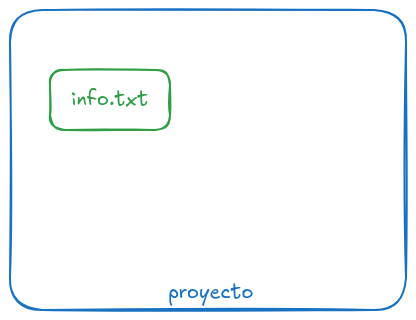
\includegraphics[width=0.95\textwidth]{graficos/carpeta.png} 
        \caption{Directorio 'proyecto' \textbf{antes} de hacer \textit{git init}}
    \end{minipage}\hfill
    \begin{minipage}{0.45\textwidth}
        \centering        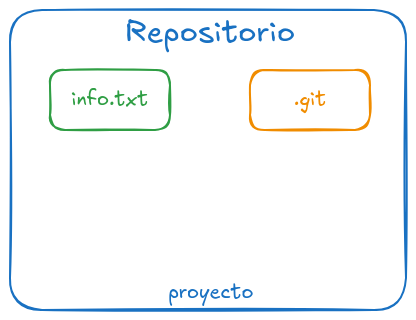
\includegraphics[width=0.95\textwidth]{graficos/Repo.png} 
        \caption{Directorio 'proyecto' \textbf{luego} de hacer \textit{git init}}
    \end{minipage}
\end{figure}

    
\end{frame}

\begin{frame}[fragile, t]{¿Está preparado, confirmado o ninguna de las dos?}
    \begin{comando}
        git status
    \end{comando}
        \begin{block}{Output de ejemplo}
            \begin{center}
            \texttt{nothing to commit (create/copy files and use "git add" to track)}
            \end{center}
        \end{block}
    \pause
    \begin{ejercicio}{Ejercicio}
        Crear un nuevo archivo en nuestro repositorio y ejecuten \textit{git status}. Vean como cambia el mensaje. Recuerden el comando \textit{touch}.
    \end{ejercicio}

\end{frame}
\begin{frame}[fragile, t]{¿Está preparado, confirmado o ninguna de las dos?}
    \begin{comando}
        git status
    \end{comando}
    \begin{block}{Output de ejemplo}
            \begin{center}
            \texttt{Untracked files:
  (use "git add <file>..." to include in what will be committed) \\archivo}
            \end{center}
        \end{block}
\begin{ejercicio}{Ejercicio}
    Ejecuten el comando que les sugiere \textit{git} para incluír el archivo que crearon recién. Hagan \textit{git status}.
\end{ejercicio}
\end{frame}


\begin{frame}{¿Está preparado, confirmado o ninguna de las dos?}
    \begin{figure}
    \centering
    \begin{minipage}{0.45\textwidth}
        \centering        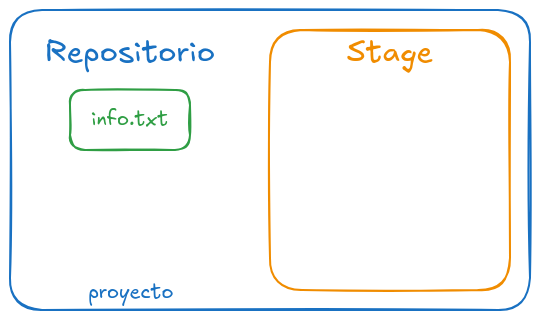
\includegraphics[width=0.95\textwidth]{graficos/stage_1.png} 
        \caption{Directorio 'proyecto' \textbf{antes} de hacer \textit{git add info.txt}}
    \end{minipage}\hfill
    \begin{minipage}{0.45\textwidth}
        \centering        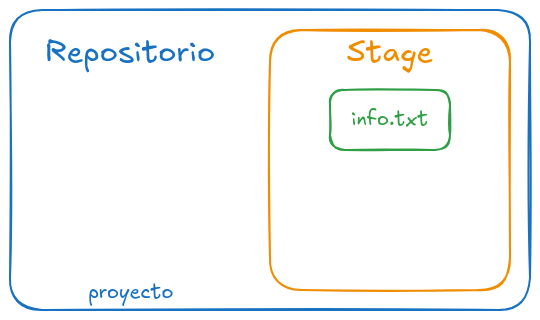
\includegraphics[width=0.95\textwidth]{graficos/stage_2.png} 
        \caption{Directorio 'proyecto' \textbf{luego} de hacer \textit{git add info.txt}}
    \end{minipage}
\end{figure}
\end{frame}

\begin{frame}[fragile, t]{¿Está preparado, confirmado o ninguna de las dos?}
    \begin{comando}
        git status
    \end{comando}
    \begin{block}{Output de ejemplo}
            \begin{center}
            \texttt{Changes to be committed:
  (use "git rm --cached <file>..." to unstage)
        \\new file:  archivo}
            \end{center}
        \end{block}
   \begin{block}{}
       Con esto vemos que \textit{git} ahora conoce al nuevo archivo, y lo va a tener en cuenta cuando hagamos un \textit{commit} proximamente.
   \end{block}     

   \pause
\end{frame}

% es como un checkpoint
\begin{frame}[t]{Confirmando cambios}
    \begin{comando}
        git commit
    \end{comando}

    \pause
    \begin{block}{}
        Una vez que tenemos ciertos cambios marcados con \textit{add}, podemos confirmarlos
        ejecutando \texttt{git commit -m "mensaje"}.

        \vspace{0.5em}

        Donde \texttt{[mensaje]} es una breve descripción de los cambios que acabamos de confirmar.
    \end{block}
    \pause
    \begin{resumen}{¡Yo elijo lo que pongo en el stage!}
        \begin{itemize}
            \item Puedo poner y sacar archivos como \textit{staged} usando \textit{git add} y \textit{git rm --cached}.
            \item Git nos sugiere estos comandos luego de hacer \textit{git status}.
        \end{itemize}    
    \end{resumen}
    \pause
    \begin{ejercicio}{Ejercicio}
        Hagan el \textit{commit} que venían preparando y elijan un mensaje. Luego hagan \textit{git status}.
    \end{ejercicio}
\end{frame}

\begin{frame}{¿Está preparado, confirmado o ninguna de las dos?}
    \begin{figure}
    \centering
    \begin{minipage}{0.45\textwidth}
        \centering        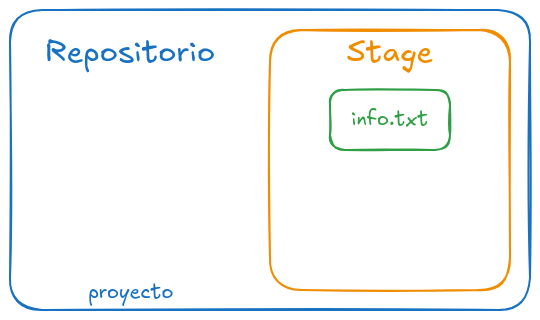
\includegraphics[width=0.95\textwidth]{graficos/stage_2.png} 
        \caption{Directorio 'proyecto' \textbf{antes} de hacer \textit{commit}}
    \end{minipage}\hfill
    \begin{minipage}{0.45\textwidth}
        \centering        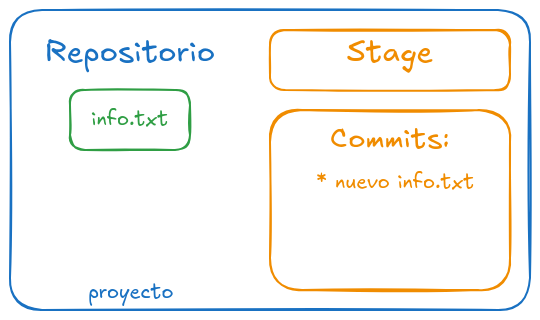
\includegraphics[width=0.95\textwidth]{graficos/commit.png} 
        \caption{Directorio 'proyecto' \textbf{luego} de hacer \textit{git commit -m "nuevo info.txt"}}
    \end{minipage}
\end{figure}
\end{frame}

\begin{frame}{¿Y si modifico el archivo luego del commit?}
    \begin{comando}
        git status
    \end{comando}
    \begin{block}{Output de ejemplo}
    \centering
        \texttt{Changes not staged for commit:\\
  (use "git add <file>..." to update what will be committed)\\
  (use "git restore <file>..." to discard changes in working directory)\\
	modified:   archivo}
    \end{block}  
\end{frame}

\begin{frame}{Elige tu propia aventura}
\begin{figure}
    \centering
    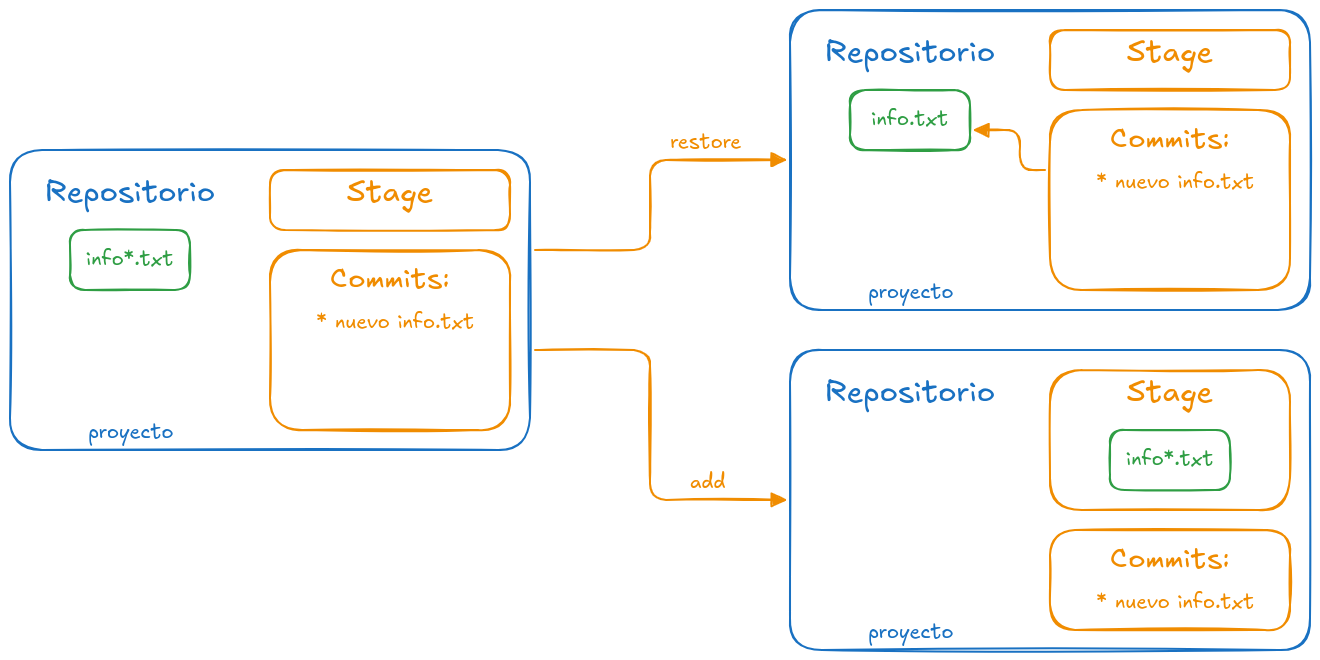
\includegraphics[width=0.99\linewidth]{graficos/restore-add.png}
    \caption{Nosotros decidimos que hacer con los nuevos cambios.
    Los añadimos al stage con \textit{add}, o los rechazamos con \textit{restore}. Tener en cuenta que al rechazar los cambios, volvemos al estado del archivo en el último commit.}
\end{figure}  
\end{frame}

\begin{frame}{Estados de un archivo}

    \begin{block}{Los cuatro estados de los archivos}
            \begin{enumerate}
    \item Untracked = Sin seguimiento
    \item Unmodified = Sin modificar
    \item Modified = Modificado
    \item Staged, to be commited = Confirmado
    \end{enumerate}
    \end{block}
    \begin{center}
        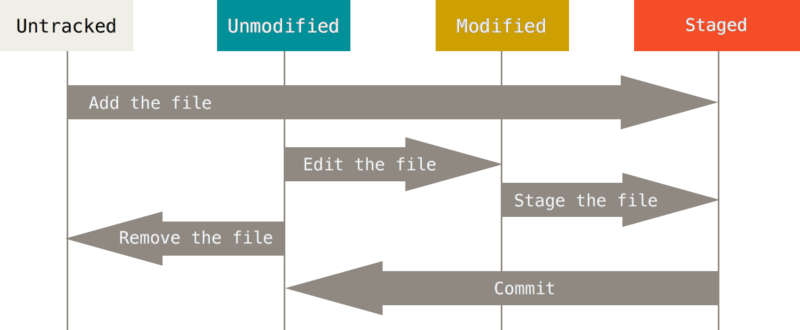
\includegraphics[width=4in]{images/lifecycle.png}
    \end{center}    
\end{frame}

% \begin{frame}[t]{¿Cómo funciona Git?}
%     \begin{center}
%         \begin{block}{Sistema de \textit{Snapshots}}
%         \begin{enumerate}
%             \item Piensa a los archivos como una serie de 'fotos'.
%             \item Con cada commit, es decir, cada vez que guardas el estado del repo, saca una 'foto' del \textit{stage} y guarda una referencia a esa foto.
%             \item Para saber el contenido de un archivo, git mira todos los commits que lo incluyan.
            
%         \end{enumerate}

%         \end{block}

%         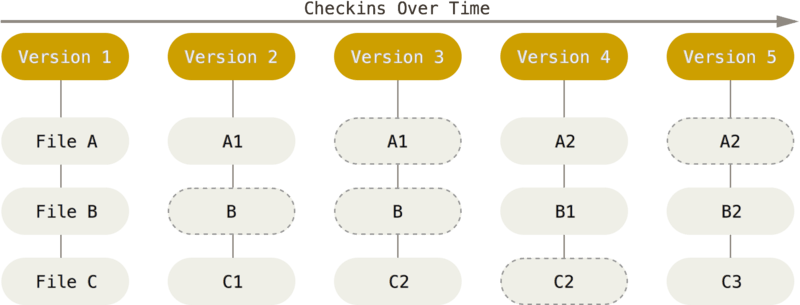
\includegraphics[width=4in]{images/snapshots.png}
%     \end{center}
    
% \end{frame}

\begin{frame}{Historial}
 \begin{comando}
     git log
 \end{comando}
 \pause
 \begin{block}{}
     Este comando nos sirve para ver el historial de cambios, o commits. Además nos dice quién hizo cada cosa, cuando, y su correo electrónico.
 \end{block}
 \pause
    \begin{figure}[ht]
        \begin{center}
            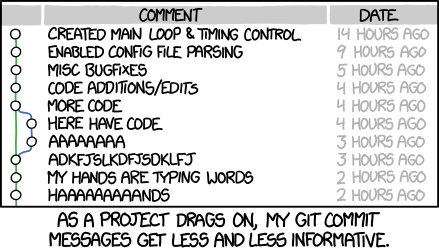
\includegraphics[height=1.7in]{images/xkcd-git-commit.png}
        \end{center}
        \caption{Fuente: \url{https://xkcd.com/1296/}}
    \end{figure}
\end{frame}

% \begin{frame}{Integrando los conceptos}
% \begin{ejercicio} {Ejercicio integrador}
%     \begin{enumerate}
%         \item En el repositorio donde venían trabajando, creen dos archivos 'pepe' y 'juan'. Recuerden el comando \textit{touch}.
%         \pause
%         \item Hagan add y commit con un mensaje como 'creación de archivos'.
%         \pause
%         \item Usando nano, escriban unas palabras acerca de pepe y juan, en sus archivos respectivos.
%         \pause
%         \item 
%         \pause
%         \item Para ver el estado final de su repo con un gráfico,\\
%         hagan \textit{git log - -graph}
%     \end{enumerate}
% \end{ejercicio}
%\end{frame}

